%======================================================
% This file is part of
% "AMCOS_booklet"
% Version 1.1 (04/07/2019)
% A LaTeX template for conference books of abstracts
%
% This template is available at:
% https://github.com/maximelucas/AMCOS_booklet
%
% License: GNU General Public License v3.0
%
% Authors:
% Maxime Lucas (ml.maximelucas@gmail.com)
% Pau Clusella
%=======================================================

\documentclass[openany, parskip=full, 12pt, a4]{scrbook}
\usepackage[margin=1in]{geometry}

%======================================================
% This file is part of
% "AMCOS_booklet"
% Version 1.1 (04/07/2019)
% A LaTeX template for conference books of abstracts
%
% This template is available at:
% https://github.com/maximelucas/AMCOS_booklet
%
% License: GNU General Public License v3.0
%
% Authors:
% Maxime Lucas (ml.maximelucas@gmail.com)
% Pau Clusella
%=======================================================

\usepackage[utf8]{inputenc}
\usepackage[T1]{fontenc}

%---------------------------------------------------------
% PACKAGES
%---------------------------------------------------------

% TYPOGRAPHY
\usepackage{xspace}
\usepackage{microtype}
\usepackage{cmbright} % different fonts

% VARIA
\usepackage{color}
\usepackage[table]{xcolor} % loads also »colortbl« %load before tikz if options
\usepackage{scrhack} % fix koma script warning about addtolist
\usepackage{blindtext}
\usepackage{pdfpages} % for cover 

\usepackage{ifthen} % to have online and printed versionw

% GRAPHICS & FIGURES & TABLES
\usepackage{graphicx}
\usepackage{float}
\usepackage{multicol} % for timetable
\usepackage{longtable} % for list of participants over more than 1 page
%\usepackage{wrapfig}
%\usepackage{tikz}
%\tikzset{ar/.style={>=latex, ->}}
%\renewcommand{\arraystretch}{1.2}
%\usepackage[multidot]{grffile}
% \usepackage{booktabs}

% WANTS TO BE LAST
\usepackage[english]{babel}

\usepackage[hidelinks]{hyperref}
\hypersetup{pdfpagelayout=TwoPageRight}
% \usepackage[ocgcolorlinks]{hyperref}
% \hypersetup{colorlinks, linkcolor={wolf}, linktocpage=true, citecolor ={tpred}, urlcolor={black}}


%-------------------------------------------------------------
% SETTINGS
%-------------------------------------------------------------
\pagestyle{plain}

\setcounter{secnumdepth}{-2} % remove numbering at any level both for the heading and the toc
%https://tex.stackexchange.com/questions/30122/generate-table-of-contents-when-section-sections-without-numbering-has-been

%-------------------------------------------------------------
% USEFUL DEFINTIONS
%-------------------------------------------------------------

% VARIA 
\newcommand\tab[1][1cm]{\hspace*{#1}}
%======================================================
% This file is part of
% "AMCOS_booklet"
% Version 1.1 (04/07/2019)
% A LaTeX template for conference books of abstracts
%
% This template is available at:
% https://github.com/maximelucas/AMCOS_booklet
%
% License: GNU General Public License v3.0
%
% Authors:
% Maxime Lucas (ml.maximelucas@gmail.com)
% Pau Clusella
%=======================================================

%
% COLORS
%

\definecolor{myorange}{RGB}{255,117,40}
\definecolor{mygray}{RGB}{164, 168, 172}
\definecolor{mywhite}{RGB}{235, 238, 231}
\definecolor{myblue}{RGB}{52, 115, 116}

\newcommand{\primarycolor}{myblue}
\newcommand{\secondarycolor}{mywhite}
\newcommand{\ternarycolor}{mywhite}

%
% BOOKLET VERSIONS
%

% If compilation is done with 'compile.sh', both versions (online and printed) are automatically compiled
% If compilation is done from editor, choose which version to compile below
\makeatletter
\@ifundefined{ifOnline}{% % check if already defined from the command line, if not define \ifOnline
	\expandafter\newif\csname ifOnline\endcsname
	\Onlinefalse %set to \Onlinefalse/\Onlinetrue for printed/online version
}{}
\makeatother

% define \type to input the right version of the abstracts
\ifOnline
\newcommand{\type}{o}
\else
\newcommand{\type}{p}
\fi % end if

%
% ABSTRACT ENVIRONMENTS
%

%----------------------------------------
% online abstract environment
%----------------------------------------
\newenvironment{abstract_online}[4] %{title}{author}{affiliation}{type}
{\filbreak %avoid page break
	
	{\large \bfseries #1}
	
	{\bfseries \itshape #2} \hfill {#3}
	
	\textcolor{mygray}{#4}
	
}
{}

%----------------------------------------
% talk abstract environment (printed)
%----------------------------------------
\newenvironment{abstract}[4] %{title}{author}{affiliation}
{\filbreak %avoid page break
	
	{\large \bfseries #1}
	
	{\bfseries \itshape #2,} \textcolor{mygray}{#3} \hfill {#4}
	
	
}
{}

%----------------------------------------
% poster abstract environment (printed)
%----------------------------------------
\newcommand{\poster}[3] %{title}{author}{affiliation}
{\filbreak %avoid page break
	
	{\bfseries \large #1} \\	
	\tab #2, \textit{#3}
	
}
{}

%----------------------------------------
% tags for talk type (colored circle in abstracts)
%----------------------------------------

\newcommand{\KLtag}{\tikz[baseline={([yshift=-.8ex]current bounding box.center)}]  \node[circle, inner sep=2pt, minimum size=0.5em, color=black, fill=\KLcolor]{\small \bfseries KL};} %colored circle with tag

\newcommand{\IStag}{\tikz[baseline={([yshift=-.8ex]current bounding box.center)}]  \node[circle, inner sep=2pt, minimum size=0.5em, color=black, fill=\IScolor]{\small \bfseries IS};} %colored circle with tag

\newcommand{\CTtag}{\tikz[baseline={([yshift=-.8ex]current bounding box.center)}]  \node[circle, inner sep=2pt, minimum size=0.5em, color=black, fill=\CTcolor]{\small \bfseries CT};} %colored circle with tag

\newcommand{\ITtag}{\tikz[baseline={([yshift=-.8ex]current bounding box.center)}]  \node[circle, inner sep=2pt, minimum size=0.5em, color=black, fill=\ITcolor]{\small \bfseries IT};} %colored circle with tag

%
% PAGE LAYOUT DEFINITIONS
%
\usepackage{etoolbox}

%------------------------------------------------------
% page style: vertical line on the side of each page
%------------------------------------------------------
\usepackage[scale=1,angle=0,opacity=1]{background}
\backgroundsetup{contents={}}

\AddEverypageHook{%
\ifthenelse{%
	\isodd{\thepage} \AND  \thepage>1 % if odd page but not front page
	}{%
	\backgroundsetup{
		color=\secondarycolor,
		position=current page.south east,%
		nodeanchor=south east,
		contents={\rule{10pt}{0.66\paperheight}}
		}
	}{%
	% nothing
	}
%
\ifthenelse{% 
	\NOT \isodd{\thepage} \AND \NOT \thepage=44% if even page
	}{%
	\backgroundsetup{
		color=\secondarycolor,
		position=current page.south west,%
		nodeanchor=south west,
		contents={\rule{10pt}{0.66\paperheight}}
		}
	}{%
	% nothing
	}
\BgMaterial}


%---------------------------------------------------
% chapter heading style
%---------------------------------------------------

\newdimen\mybarpadding
\mybarpadding=1.5em\relax %padding between gcolored bar and chapter name

\RedeclareSectionCommand[%
    ,afterskip=4em plus 1pt minus 1pt%
    ,beforeskip=-1pt%1.2em plus 1pt minus 1pt%
    ,level=0%
    ,toclevel=0%
]{chapter}%

\setkomafont{chapter}{\normalfont\normalsize\bfseries\Huge} % koma-script-specific command

\newcommand*{\mynumberedtest}[1]{% to test whether there is a number
  \if\relax\detokenize{#1}\relax%
  \else%
    #1%
    
  \fi}

%-------------------------------------------------chapter style definition

\renewcommand{\chapterlinesformat}[3]{%
  \Ifthispageodd{%
    \hfill%
    \raisebox{-0.2em}{%
      \makebox[0pt][r]{\textcolor{\primarycolor}{\rule{\paperwidth}{1em}}}%
    }%
    \hspace{\mybarpadding}%
% 	\mynumberedtest{#2}
	\mbox{#3}%
  }{%
%    \hbox{%
%       \mynumberedtest{#2}
      \mbox{#3}%
      \hspace{\mybarpadding}%
      \raisebox{-0.2em}{%
        \makebox[0pt][l]{\textcolor{\primarycolor}{\rule{\paperwidth}{1em}}}%
      }%
%    }%
  }%
}
\makeatother
%---------------------------------------------------------

% TIMETABLE COLORS AND STYLES

% text and backgroud colors
\newcommand{\tbg}{gray} % background
\newcommand{\tfg}{white}
\newcommand{\tbc}{gray!25}

% talk types colors
\newcommand{\IScolor}{myblue!65} % invited speaker
\newcommand{\CTcolor}{white} % contributed talk
\newcommand{\KLcolor}{myorange!45} % keynote lecture
\newcommand{\ITcolor}{yellow!25} %

% row types
\newcommand{\tablebreak}[2]{% {time span}{break name}
	\rowcolor{\tbc} #1 &  \multicolumn{4}{c|}{\bfseries #2} \\ \hline }
\newcommand{\eventtype}[2]{% {time span}{event name}
	#1& \multicolumn{4}{c|}{\cellcolor{\tbg}\color{\tfg}\bfseries #2} \\ \hline }

% column spacing and position
\newcolumntype{L}[1]{%
	>{\raggedright\let\newline\\\arraybackslash\hspace{0pt}}m{#1}}
\newcolumntype{C}[1]{%
	>{\centering\let\newline\\\arraybackslash\hspace{0pt}}m{#1}}
\newcolumntype{R}[1]{%
	>{\raggedleft\let\newline\\\arraybackslash\hspace{0pt}}m{#1}}

%\newcommand{\mytable}{|C{0.15\linewidth}| C{0.05\linewidth}|  C{0.25\linewidth} C{0.1\linewidth} C{0.5\linewidth}|}

\newcommand{\IS}[5]{% {time span}{name}{University}{City, Country}{title}
	#1 &\cellcolor{\IScolor}IS&{\bfseries#2}\newline #4&&#5 \\ \hline}
\newcommand{\CT}[5]{%
	#1 &\cellcolor{\CTcolor}CT&{\bfseries#2}\newline #4&&#5 \\ \hline}
\newcommand{\KL}[5]{%
	#1 &\cellcolor{\KLcolor}KL&{\bfseries#2}\newline #4&&#5 \\ \hline}
\newcommand{\IT}[5]{%
	#1 &\cellcolor{\ITcolor}IT&{\bfseries#2}\newline #4&&#5 \\ \hline}
\newcommand{\tutorial}[5]{%
	#1 && {\bfseries#2}\newline #4 &&#5 \\ \hline}

\begin{document}

% COVER PAGE
%--------------------------------------------------------------------
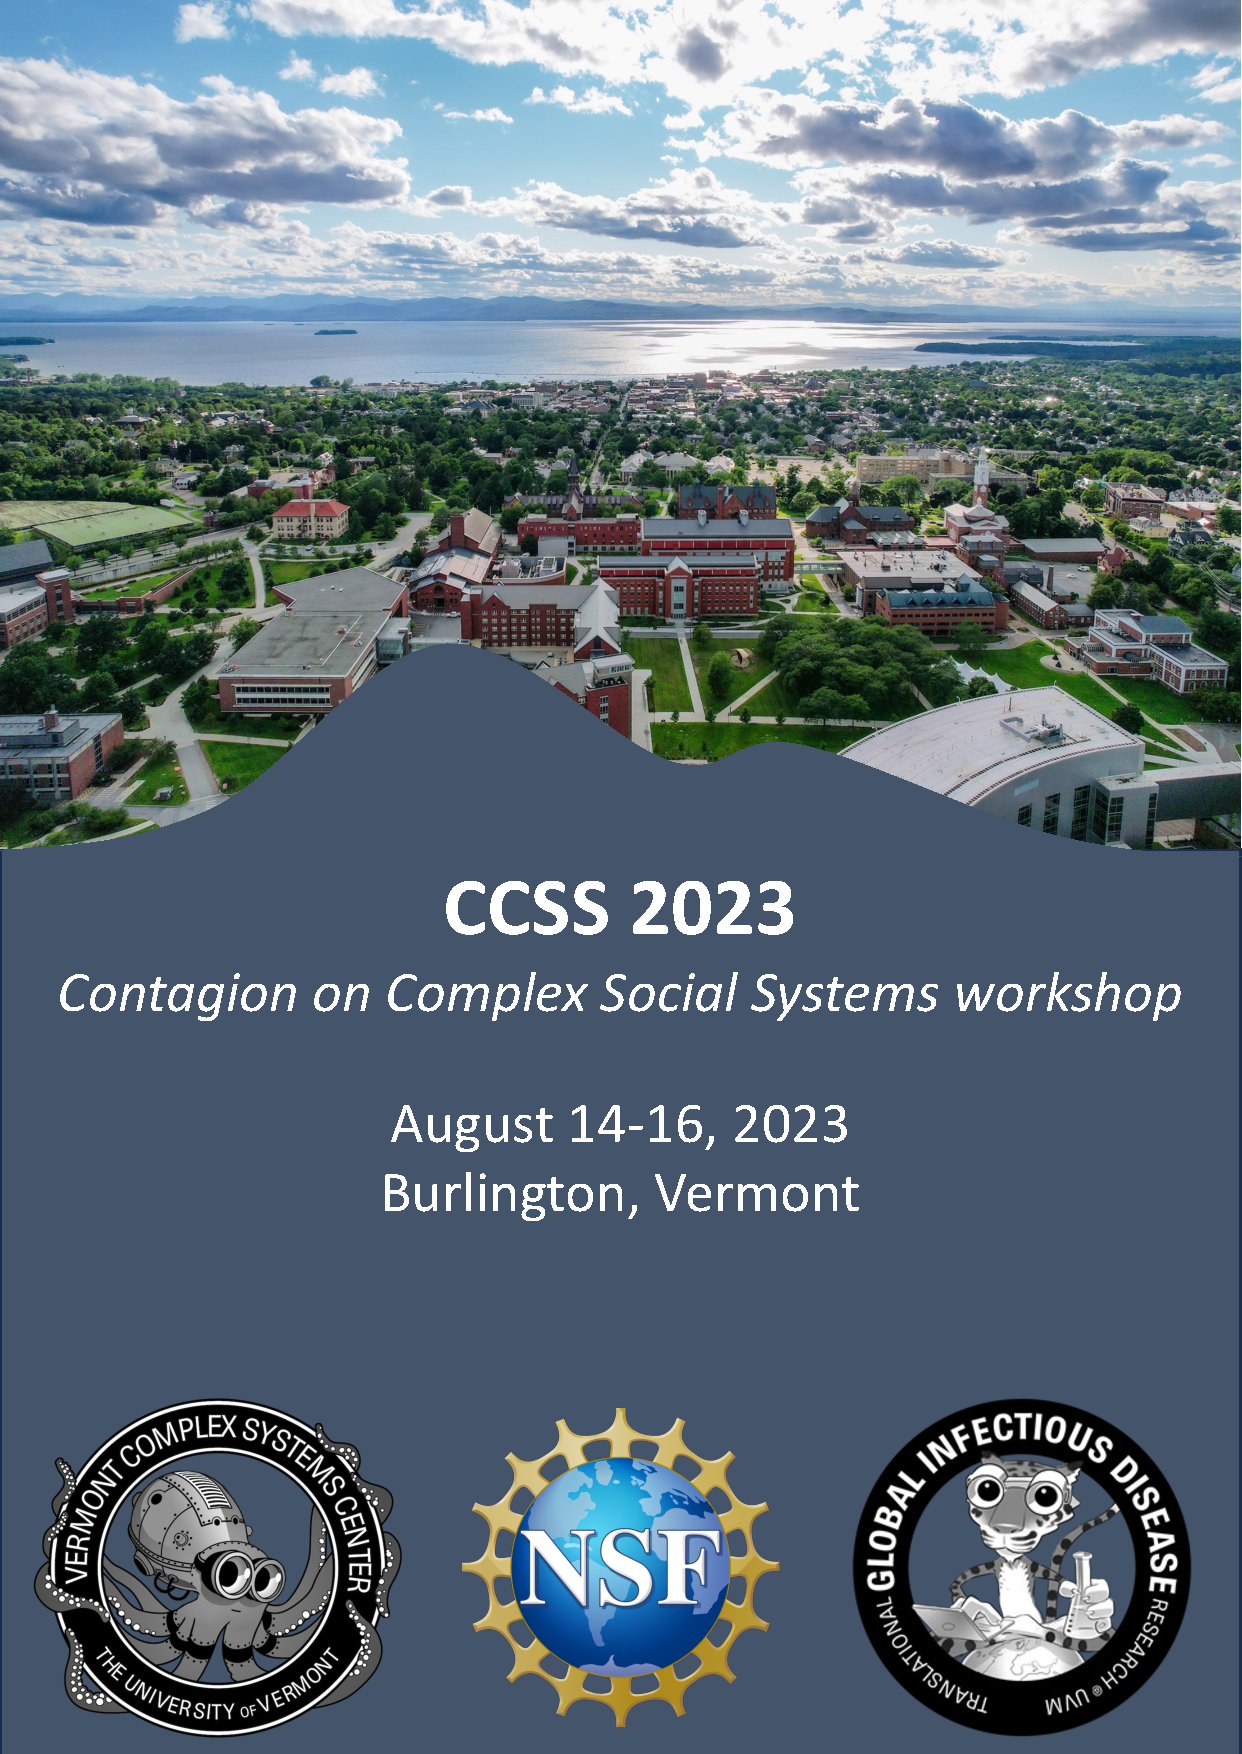
\includepdf{images/cover.pdf}	% our cover was produced with canva.com
	
	
% BLANK PAGE
%---------------------------------------------------------------------
\mbox{}
\thispagestyle{empty}
\vfill
\begin{center}
The open-source \LaTeX{} template, \verb"AMCOS_booklet", used to generate this booklet is available at \url{https://github.com/maximelucas/AMCOS\_booklet}
\end{center}

\newpage

% TABLE OF CONTENTS 
%---------------------------------------------------------------------
\tableofcontents

% ABOUT
%---------------------------------------------------------------------
\chapter{About}

Contagion on Complex Social Systems (CCSS) 2023 is an interdisciplinary workshop gathering world leaders and young researchers in topics related to modeling of contagion in social systems in order to promote and cross-fertilize various computational and modeling approaches.

\section{Organizing committee}

\begin{itemize}
    \item Nicholas Landry, University of Vermont
    \item Jean-Gabriel Young, University of Vermont
    \item Juan G. Restrepo, University of Colorado Boulder
    \item jimi adams, University of Colorado Denver
    \item Laurent Hébert-Dufresne, University of Vermont
    \item Alice Schwarze, Dartmouth College
\end{itemize}

% TIMETABLE 
%---------------------------------------------------------------------
\chapter{Timetable}

CT: Contributed Talk, IT: Invited Talk.


\section{Monday, August 14th}
\begin{center}
	\filbreak
\begin{longtable}{|C{0.15\linewidth}| C{0.04\linewidth}|  C{0.3\linewidth} C{0.0\linewidth} C{0.4\linewidth}|}\hline	
	\tablebreak{8:00--9:00}{Registration and Coffee}
	\tablebreak{9:00--9:10}{Welcome remarks}
	\tablebreak{}{Morning Session Chair: Nicholas Landry}
	\IT{9:10--10:10}{Caroline Buckee}{}{Harvard}{TBD}
	\tablebreak{10:10--10:30}{Coffee break}
	\CT{10:30-10:45}{Mariah Boudreau}{}{Vermont}{Sensitivity analysis of stochastic polynomials, and its application to epidemic forecasting and random graphs}
	\CT{10:45:-11:00}{Yassin Bahid}{}{CU Boulder}{The statistical and dynamic modeling of protests in Ukraine: the revolution of dignity and preceding times}
	\CT{11:00-11:15}{Anjalika Nande}{}{Johns Hopkins}{Factors affecting variant invasion and spread in an ongoing epidemic}
	\tablebreak{11:15--11:30}{Break}
	\CT{11:30-11:45}{Changqing Cheng}{}{Binghamton}{Multilayer networks with higher-order interaction reveal the impact of collective behavior on epidemic dynamics}
	\CT{11:45-12:00}{jimi adams}{}{CU Denver}{Peer Network Processes in Adolescents' Health Lifestyles}
	\tablebreak{12:00--14:00}{Lunch (on your own)}
	\tablebreak{}{Afternoon Session Chair: Mariah Boudreau}
	\IT{14:00--15:00}{Michael Johansson}{}{CDC}{TBD}
	\tablebreak{15:00--15:30}{Coffee Break}
	\CT{15:30-15:45}{Senay Yitbarek}{}{UNC Chapel Hill}{TBD}
	\CT{15:45-16:00}{Guillaume St-Onge}{}{Northeastern}{Probability generating functions for epidemics on metapopulation networks}
	\CT{16:00-16:15}{Corbit Sampson}{}{CU Boulder}{Competing Social Contagions with Opinion Dependent Infectivity}
	\tablebreak{16:15--17:00}{Discussion}
	\tablebreak{17:00}{Dinner (on your own)}
\end{longtable}
\end{center}

\newpage
\section{Tuesday, August 15th}
\begin{center}
	\begin{longtable}{|C{0.15\linewidth}| C{0.04\linewidth}|  C{0.3\linewidth} C{0.0\linewidth} C{0.4\linewidth}|}\hline
		\tablebreak{}{Morning Session Chair: Anjalika Nande}
		\IT{9:00--10:00}{Sandra González-Bailón}{}{Penn}{TBD}
		\tablebreak{10:00--10:30}{Coffee Break}
		\CT{10:30-10:45}{Sam Scarpino}{}{Northeastern}{Crowding and shape of epidemics}
		\CT{10:45:-11:00}{Maximilian Nguyen}{}{Princeton}{Fundamental Bound on Epidemic Overshoot in the SIR Model}
		\CT{11:00-11:15}{Aparna Ananthasubramaniam}{}{Michigan}{Networks and Identity Drive Geographic Properties of the Diffusion of Lexical Innovation}
		\tablebreak{11:15--11:30}{Break}
		\CT{11:30-11:45}{Maisha Sejunti}{}{SUNY Buffalo}{Floquet Theory for Spreading Dynamics over Periodically Switching Networks}
		\CT{11:45-12:00}{Zhen Guo}{}{Northeastern}{Fandom Brokerage: Contagion from Twitter to Chinese Social Media}
		\tablebreak{12:00--14:00}{Lunch (on your own)}
		\tablebreak{}{Afternoon Session Chair: jimi adams}
		\IT{14:00--15:00}{C. Brandon Ogbunu}{}{Yale}{TBD}
		\tablebreak{15:00--15:30}{Coffee Break}
		\CT{15:30-15:45}{Subekshya Bidari}{}{Columbia}{Measles transmission in household structured models}
		\CT{15:45-16:00}{Katherine Betz}{}{SUNY Buffalo}{Multi-Population Evolutionary Game Dynamics on Networks}
		\CT{16:00-16:15}{Chadi Saad-Roy}{}{UC Berkeley}{Modelling SARS-CoV-2 immuno-epidemiological dynamics}
		\tablebreak{16:15--17:00}{Discussion}
		\tablebreak{17:00}{Dinner (on your own)}
	\end{longtable}
\end{center}

\newpage
\section{Wednesday, August 16th}
\begin{center}
	\begin{longtable}{|C{0.15\linewidth}| C{0.04\linewidth}|  C{0.3\linewidth} C{0.0\linewidth} C{0.4\linewidth}|}\hline
		\tablebreak{}{Morning Session Chair: Aparna Ananthasubramaniam}
		\IT{9:00--10:00}{Tim Waring}{}{Maine}{TBD}
		\tablebreak{10:00--10:30}{Coffee Break}
		\CT{10:30-10:45}{Daniel Cooney}{}{Penn}{Social Dilemmas of Sociality due to Beneficial and Costly Contagion}
		\CT{10:45:-11:00}{Juanjuan Zhang}{}{Fudan University}{Heterogeneous changes in mobility in response to the SARS-CoV-2 Omicron BA.2 outbreak in Shanghai}
		\CT{11:00-11:15}{Amanda McGowan}{}{Concordia}{Networks of wellness}
		\tablebreak{11:15--16:00}{Discussion}
		\tablebreak{12:00--14:00}{Lunch}
		\tablebreak{}{Afternoon Session Chair: Jean-Gabriel Young}
		\IT{14:00--15:00}{Sarah Nowak}{}{Vermont}{TBD}
		\tablebreak{15:00--15:30}{Coffee Break}
		\CT{15:30-15:45}{Ayush Chopra}{}{MIT}{Learning to Simulate Millions of Agents by bridging AI and Agent- based Models}
		\CT{15:45-16:00}{Andrés Colubri}{}{UMass Chan Medical School}{TBD}
		\tablebreak{15:00--15:30}{Closing Remarks}
	\end{longtable}
\end{center}

% TALKS 
%---------------------------------------------------------------------
\chapter{List of Abstracts}

\section{Monday, August 14th}

% % Definitions of custom environment used here can be found in preamble_booklet.tex file

% % The following input commands automatically select the right version 
% % (print or online) version of the abstract's .tex
% % \type is defined in preamble_booklet.tex and equals:
% % 'o' (online) or 'p' (print)

    \begin{abstract_online}{None}{%
        C. Buckee}{%
        }{%
        Harvard University, Boston, MA}
    None  
    
    \end{abstract_online}
    

    \begin{abstract_online}{Sensitivity analysis of stochastic polynomials, and its application to epidemic forecasting and random graphs}{%
        M. Boudreau}{%
        }{%
        University of Vermont, Burlington, VT}
    Probability generating functions (PGFs) provide an analytical and probabilistic description of random networks. In the context of emerging infectious diseases and their transmission trees, PGFs become a powerful tool for probabilistic forecasting that naturally accounts for the intrinsic stochasticity of disease transmission. However, transmission trees are incredibly noisy data as they either come from genomic sequencing with imperfect sampling or contact tracing in noisy environments. It is therefore critical to evaluate the importance of data quality for probabilistic forecasts made with PGFs.  This research explores the variation in final epidemic size for various degree distributions (i.e. distributions of secondary infections per case)  and associated parameters given different levels of added error. The objective is to characterize the sensitivity to noise of PGFs in different network conditions. Preliminary results show larger uncertainty when adding error to more homogeneous degree distributions, suggesting that the PGF framework might be better suited for diseases transmitted through direct contact rather than airborne infections, as the former tends to show more heterogeneous transmission patterns. Altogether, this project paves the way towards a noisy and probabilistic forecasting framework for emerging epidemics while taking into account confidence in data and a network’s noise sensitivity. 
    
    \end{abstract_online}
    

    \begin{abstract_online}{The statistical and dynamic modeling of protests in Ukraine: the revolution of dignity and preceding times}{%
        Y. Bahid}{%
        }{%
        University of Colorado Boulder, Boulder, CO}
    Ukraine's tug-of-war between Russia and the West has had significant and lasting consequences for the country.  In 2013 the Russian-leaning Ukrainian president, Viktor Yanukovych,  refused to sign the association agreement with the European Union. This led to widespread protests centered in Kyiv's Maidan Square.  The protests went on to be known as the Euromaidan protests.  In this work, we analyze open 2013 protest data  from the Center for Social and Labor Research in Ukraine.  Our analysis shows that there is self-excitation in the system even before the Euromaidan protests began and this self-excitation magnifies during the Euromaidan protests.  Our statistical analysis suggests that the government's use of force is associated with more future protests, having an inflammatory rather than suppressing effect on protests. Furthermore, we introduce Hawkes process models to understand the spatiotemporal dynamics of the protesting activity.  We find that while the protest activity spread throughout the country the dynamics of the protests were driven by Kyiv's level of activity.  Moreover, while previous work has shown that geographical proximity is a significant predictor of the spread of events, our work illustrates that the political affinity between oblasts was a far more significant factor than the geographical distance between oblasts in determining the spread of protests. This highlights the importance of social and cultural factors in shaping the dynamics of political movements. 
    
    \end{abstract_online}
    

    \begin{abstract_online}{Factors affecting variant invasion and spread in an ongoing epidemic}{%
        A. Nande}{%
        }{%
        Johns Hopkins University, Baltimore, MD}
    The COVID-19 pandemic has been characterized by variants of concern that have exhibited varying degrees of transmissibility and evasion from infection and vaccine acquired immunity. Although a lot of work has been done to characterize these phenotypes, the factors that affect selection and competition between different strains ­– which in turn govern the dynamics of their spread ­– are not well understood. In this study we use a stochastic two strain SIR model with a resident and a variant strain to analyze how the variant type (increased transmissibility or immune evasion), time of variant introduction, and the contact network structure affect the ability of a variant to invade and spread in the population. We find that apart from strains that are highly immune evasive, variants that are introduced later in an epidemic find it harder to invade. For strains that successfully invade, a variant with transmission advantage quickly increases in prevalence, and the rate at which it takes over the resident strain is faster the earlier it is introduced. Immune evasive variants on the other hand can linger at a low prevalence for a long time and increase in prevalence only after they have sufficient fitness advantage due to a build-up of immunity to the resident strain. This highlights that immune evasive variants produced during the early stages of an epidemic may not be observed until much later. We also investigate the role played by the transmission network structure, focusing on the effects of superspreading and clustering. Although inspired by the current pandemic, our approach is general and highlights some important characteristics of variant spread. Future work will consider a COVID-19 specific model to better understand the spread of Delta and Omicron, as well as to identify the types of variants that might dominate in the future. 
    
    \end{abstract_online}
    

    \begin{abstract_online}{Multilayer networks with higher-order interaction reveal the impact of collective behavior on epidemic dynamics}{%
        C. Cheng}{%
        }{%
        Binghamton University, Binghamton, NY}
    The ongoing COVID-19 pandemic has inflicted tremendous economic and societal losses. In the absence of pharmaceutical interventions, the population behavioral response, including situational awareness and adherence to non-pharmaceutical intervention policies, has a significant impact on contagion dynamics. Game-theoretic models have been used to reproduce the concurrent evolution of behavioral responses and disease contagion, and social networks are critical platforms on which behavior imitation between social contacts, even dispersed in distant communities, takes place. Such joint contagion dynamics has not been sufficiently explored, which poses a challenge for policies aimed at containing the infection. In this study, we present a multi-layer network model to study contagion dynamics and behavioral adaptation. It comprises two physical layers that mimic the two solitary communities, and one social layer that encapsulates the social influence of agents from these two communities. Moreover, we adopt high-order interactions in the form of simplicial complexes on the social influence layer to delineate the behavior imitation of individual agents. This model offers a novel platform to articulate the interaction between physically isolated communities and the ensuing coevolution of behavioral change and spreading dynamics. The analytical insights harnessed therefrom provide compelling guidelines on coordinated policy design to enhance the preparedness for future pandemics. 
    
    \end{abstract_online}
    

    \begin{abstract_online}{Peer Network Processes in Adolescents’ Health Lifestyles}{%
        j. adams}{%
        }{%
        University of Colorado Denver, Denver, CO}
    Combining theories of health lifestyles—interrelated health behaviors arising from group-based identities—with those of network and behavior change, we investigated network characteristics of health lifestyles and the role of influence and selection processes underlying these characteristics. We examined these questions in two high schools using longitudinal, complete friendship network data from the National Longitudinal Study of Adolescent to Adult Health. Latent class analyses characterized each school’s predominant health lifestyles using several health behavior domains. School-specific stochastic actor-based models evaluated the bidirectional relationship between friendship networks and health lifestyles. Predominant lifestyles remained stable within schools over time, even as individuals transitioned between lifestyles. Friends displayed greater similarity in health lifestyles than nonfriend dyads. Similarities resulted primarily from teens’ selection of friends with similar lifestyles but also from teens influencing their peers’ lifestyles. This study demonstrates the salience of health lifestyles for adolescent development and friendship networks. 
    
    \end{abstract_online}
    


    \begin{abstract_online}{Advances and Challenges for Infectious Disease Forecasting }{%
        M. Johansson}{%
        }{%
        Centers for Disease Control and Prevention, Atlanta, GA}
    Infectious disease forecasting has moved from an academic exercise to reality in the past decade. Real-time probabilistic forecasts have enabled the evaluation and comparison of forecast models, leading to insights on the rapid deterioration of forecast skill as forecast horizons increase, the value of ensemble forecasts, and the importance of simple baseline models. However, many challenges have also become clearer. Comparing forecast skill to benchmarks and between models with proper scores is now routine, but how good is the current best forecast? Can it be improved? What is its value to public health? How can we build an evidence base of forecast reliability? Are forecasts improving? What are the key components for better forecasts? What is needed to extend forecast horizons while maintaining reliability? What is the value of specific datasets? How can behavior and immunity be monitored and integrated? 
    
    \end{abstract_online}
    

    \begin{abstract_online}{The Truth is the Whole: Social-ecological determinants of mosquito burden in urban environments}{%
        S. Yitbarek}{%
        }{%
        University of North Carolina at Chapel Hill, Chapel Hill, NC}
    The distribution of mosquitoes and associated vector diseases (e.g., West Nile, dengue, and Zika viruses) is likely a function of environmental conditions in the landscape. Urban environments are highly heterogeneous in the amount of vegetation, standing water, and concrete structures covering the land at a given time, each having the capacity to influence mosquito abundance and disease transmission. Here, we present a meta-analysis of 42 paired observations from 18 articles testing how socioeconomic status relates to overall mosquito burden in urban landscapes in the US. We also analyzed how with socio-ecological covariates (e.g., abandoned buildings, vegetation, education, and garbage containers) varied across socioeconomic status in the same mosquito studies. The meta-analysis revealed that lower-income neighborhoods (regions with median household incomes $<$\$50,000 household-1 year-1) are exposed to 63\% greater mosquito densities and mosquito-borne illnesses compared to higher-income neighborhoods ($\geq$\$50,000 household-1 year-1). One common species of urban mosquito (Aedes aegypti) showed the strongest relationship with socioeconomic status, with Ae. aegypti being 126\% higher in low-income than high-income neighborhoods. We also found that certain socio-ecological covariates correlated with median household income. Garbage, trash, and plastic containers were found 67\% higher in low-income neighborhoods, whereas high-income neighborhoods tended to have higher levels of education. Together, these results indicate that socio-ecological factors can lead to disproportionate impacts of mosquitoes on humans in urban landscapes. Thus, concerted efforts to manage mosquito populations in low-income urban neighborhoods are required to reduce mosquito burden for the communities most vulnerable to human disease. 
    
    \end{abstract_online}
    

    \begin{abstract_online}{Probability generating functions for epidemics on metapopulation networks}{%
        G. St-Onge}{%
        }{%
        Northeastern University, Boston, MA}
    Models of contagion on metapopulation networks are effective at assessing the cryptic transmission phase at the beginning of an outbreak when data are scarce and the epidemic is driven by long-range mobility patterns. However, metapopulation frameworks either describe the average state of the system or rely on costly large-scale simulations, which take time and resources to deploy during emergent disease outbreaks. Here, we provide a flexible and computationally efficient alternative to describing the early phase of an emerging outbreak by leveraging probability generating functions (PGFs). We map the system of mobile agents (and potential carriers of diseases) to a multitype branching process (Fig. 1A), from which we can probe full probability distributions. To give a sense of scale, we get similar results to stochastic simulations in a matter of seconds, as opposed to hours of computation on supercomputers. We are able to estimate important quantities, like the current (and future) state of an outbreak (Fig. 1B), and to perform exact Bayesian inference, like in Fig. 1C where we show a posterior distribution on the basic reproduction number and the time of onset of an epidemic. Other important applications include inferring the location of the source of an outbreak, defining more constrained prior distributions for large-scale simulations, and performing an early assessment of changes in the mobility of individuals. Altogether, our approach provides timely situational awareness when the spreading of concerning diseases is detected and we plan to leverage its computational advantage to help design more robust global surveillance systems. 
    
    \end{abstract_online}
    

    \begin{abstract_online}{Moving Beyond Diffusion to Communication in Models of Information Spread}{%
        S. Kumar}{%
        }{%
        Northeastern University, Boston, MA}
    There seems to be a broadly accepted and championed notion that misinformation is analogous to an infectious disease. The position that information spreads similarly to a virus in a population is at the heart of broad swaths of behavioral science, including models of intervention acceptance and optimal advertising. While useful in some contexts, dynamical models of information diffusion built on this assumption experimentally have extremely limited predictive power. A moment’s thought elucidates the wrought oversimplification in this model–a virus spreads among hosts approximately as a replication or diffusion process, while "information" spreads as stories among interlocutors as a communication process. This work thus aims at paving a way forward towards more accurate, mechanistic, experiment-driven models of information spread. We begin by exposing the underlying suppositions of these disease-spreading models of information diffusion and consider their shortcomings in the literature and through toy models. From this basis, we are able to disentangle "information" as it was described by Shannon from the information described in diffusion models and from that which spreads qua communication. Finally, we synthesize these key considerations in the dynamics and characterization of information spread to posit a model-building framework which is grounded in a systems approach to communication, and which emphasizes the importance of novel measurement and representation techniques alongside ethnographic, pragmatic, and rhetorical analysis. 
    
    \end{abstract_online}
    


\section{Tuesday, August 15th}

    \begin{abstract_online}{TBD}{%
        S. González-Bailón}{%
        }{%
        University of Pennsylvania, Philadelphia, PA}
    TBD  
    
    \end{abstract_online}
    

    \begin{abstract_online}{Emerging call for action: The complex and paradoxical co-evolution of contagions and institutions}{%
        J. St-Onge}{%
        }{%
        University of Vermont, VT}
    Epidemic models are used to study the spread of an undesired agent through a population, be it diseases infecting countries, misinformation adulterating social media, or pests blighting regions. In fighting these epidemics, we do not exclusively depend on either global top-down interventions or individual adaptations. Interventions often come from local institutions such as public health departments, moderation teams on social media, or other forms of group governance. We leverage recent development of institutional dynamics to investigate the intermediary scale of groups, which is understudied compared to macro-level top-down interventions or micro-scale adaptive individual behaviour. Using principles adapted from group selection theory, we model meso-scale groups attempting local control of an epidemic through adaptation based on successes and failures of other groups. This modeling approach results in a hypergraph model where institutions can emerge and grow on hyperedges (representing groups) to locally affect the epidemic dynamics. In this model, we find complex co-evolutionary dynamics which we summarize as five possible dynamical regimes (see figure). Across all regimes, we find that a faster rate of policy imitation leads to a higher steady-state prevalence. Fast imitation is beneficial in the early phase, but high reactivity does not give enough time for stronger policies to prove their efficacy, eventually leading to an abundance of weak institutions unable to control the epidemic. Additionally, the initial conditions determine the transient behaviors. In particular, if groups with stronger policies are present from the outset, the magnitude of epidemic waves is greatly reduced and slightly delayed in time. Altogether our results illustrate the complex dynamics missed by models that ignore the dynamical interplay of contagions with group interventions. 
    
    \end{abstract_online}
    

    \begin{abstract_online}{Fundamental Bound on Epidemic Overshoot in the SIR Model}{%
        M. Nguyen}{%
        }{%
        Princeton University, Princeton, NJ}
    We derive an exact upper bound on the epidemic overshoot for the Kermack-McKendrick SIR model. This maximal overshoot value of 0.2984... occurs at $R_0 = 2.151\dots$. Using the general analysis framework presented within, we then consider more complex SIR models, such as those that incorporate vaccination or contact heterogeneity. We analyze models that consider vaccinations and show that the presence of vaccinated individuals decreases the maximum possible overshoot. For epidemics where the contact structure is given by a network, we numerically find that increased contact heterogeneity lowers the maximal overshoot value and weakens the dependency of overshoot on transmission. 
    
    \end{abstract_online}
    

    \begin{abstract_online}{Networks and Identity Drive Geographic Properties of the Diffusion of Lexical Innovation}{%
        A. Ananthasubramaniam}{%
        }{%
        University of Michigan, Ann Arbor, MI}
    The adoption of cultural innovation (e.g., music, beliefs, language) is often geographically correlated, with adopters largely residing within the boundaries of relatively few well-studied, socially significant areas. These cultural regions are often hypothesized to be the result of either (i) identity performance driving the adoption of cultural innovation, or (ii) homophily in the networks underlying diffusion. In this study, we show that demographic identity and network topology are both required to model the diffusion of innovation, as they play complementary roles in producing its spatial properties. We develop an agent-based model of cultural adoption, and validate geographic patterns of transmission in our model against a novel dataset of innovative words that we identify from a 10% sample of Twitter. Using our model, we are able to directly compare a  model of diffusion that combines network (homophily) and identity (performance) against simulated network-only and identity-only counterfactuals---allowing us to test the separate and combined roles of network homophily and identity performance. While social scientists often treat either network or identity as the core social structure in modeling culture change, we show that key geographic properties of diffusion actually depend on both factors as each one influences different mechanisms of diffusion. Specifically, homophily in the network principally drives spread among urban counties via weak-tie diffusion, while identity performance plays a disproportionate role in transmission among rural counties via strong-tie diffusion. Diffusion between urban and rural areas, a key component in innovation diffusing nationally, requires both network and identity. Our work suggests that models must integrate both factors in order to understand and reproduce the adoption of innovation. 
    
    \end{abstract_online}
    

    \begin{abstract_online}{Floquet Theory for Spreading Dynamics over Periodically Switching Networks}{%
        M. I. Sejunti}{%
        }{%
        State University of New York at Buffalo, Buffalo, NY}
    In many social, physical, and biological networks, their structure evolves over time with daily, weekly and/or annual cycles. For example, a college's class schedule is usually organized in weekly periodic cycles.  Thus motivated, we formulate and analyze a susceptible-infectious-susceptible (SIS) epidemic model over temporal networks with  periodically switching connections.  Using Floquet theory --- a framework that extends the theory of linear systems to the setting of time-varying periodic systems --- we characterize the epidemic threshold and growth/decay rates in terms of the Floquet exponent of a system's monodromy matrix. We further employ this framework to identify and study a Parrondo's paradox for  epidemic spreading, whereby a temporal network can have subcritical (epidemic decay) dynamics even if it seemingly appears to be super-critical (epidemic growth) at all instantaneous time (i.e., ignoring that the network is periodically switching). 
    
    \end{abstract_online}
    

    \begin{abstract_online}{Fandom Brokerage: Contagion from Twitter to Chinese Social Media}{%
        Z. Guo}{%
        }{%
        Northeastern University, Boston, MA}
    This study investigates the phenomenon that Chinese fans repost fans contents of a Thai drama from Twitter to a Chinese social media. Through qualitative analysis of Red posts featuring Twitter screenshots, the study seeks to identify the contents that are carried from outside to inside of China via fan-mediated exchanges. Patterns of contents shared are examined to highlight the impact of fandom on culture contagion. Once the fan brokerage pathway is established, it is hypothesized that content beyond the drama itself, such as LGBTQ knowledge, can also be transmitted. The findings of this study could inform future research on information brokerage in the context of pop culture and transnational social media. 
    
    \end{abstract_online}
    


    \begin{abstract_online}{TBD}{%
        C. B. Ogbunu}{%
        }{%
        Yale University, New Haven, CT}
    TBD  
    
    \end{abstract_online}
    

    \begin{abstract_online}{Measles Transmission in household structured models}{%
        S. Bidari}{%
        }{%
        Columbia University, New York, NY}
    Households are known to have a significant impact on the transmission of many diseases, yet its impact has not been fully accounted for in commonly used compartmental models. Many studies on models of disease transmission with household level mixing consider a static household distribution. These approaches have provided valuable insights on final epidemic sizes, threshold parameters, and vaccination policies but fail to consider the demographic changes in household structure for endemic diseases like measles. To capture the long-term evolution of households and dynamics of disease transmission within them, we introduce a model of disease transmission that includes demographic changes in the household sizes. We explore the variation in transmission dynamics caused by the differential changes in contact networks and population demographic over several decades of measles persistence in China. Using model simulations, we show that incorporating only age structured mixing systematically overestimate the infection compared to the models with both household and age structured mixing. Our model provides a comprehensive framework to understand the spread and endemicity of measles by incorporating household level mixing in populations without detailed household level data. 
    
    \end{abstract_online}
    

    \begin{abstract_online}{Multi-Population Evolutionary Game Dynamics on Networks}{%
        K. Betz}{%
        }{%
        University at Buffalo, SUNY, Buffalo, NY}
    Evolutionary game dynamics is the study of population change based on successful, or unsuccessful, strategies.  This exploration is often done on one population with a variety of possibilities to adjust the model in order to create an accurate representation of the natural world.  One method is the inclusion of strategy-dependent feedback.  We will explore environmental feedback, which is how the environment changes based on player actions.  While this has been done previously and in many differing circumstances, we instead explore the population dynamics for more than one population that can be modeled as a network.  This type of model, while originally examined in terms of cooperators or defectors, can easily be examined in terms of how a contagion spreads through a population. Using game theory, we can create environmentally dependent payoff matrices and feedback equations for each node, and the entire population, to use for the derivation of the full system.  Then, using replicator dynamics, we can create a model for the base case of two populations interacting and explore the subsequent system of differential equations to examine the possible equilibrium and their stability.  We find that the stability of the equilibrium is dependent on the interaction between the populations, which tells us that the rate of interaction can change the population equilibrium.  In terms of a contagion, the rate of interaction can change the frequency of infected in each population.  Thus, using evolutionary game dynamics, we explore the system of equations and examine equilibrium and their stability requirements to model the change of the frequency of strategies in two interacting populations. 
    
    \end{abstract_online}
    

    \begin{abstract_online}{Modelling SARS-CoV-2 immuno-epidemiological dynamics}{%
        C. Saad-Roy}{%
        }{%
        University of California Berkeley, Berkeley, CA}
    The COVID-19 pandemic is a global emergency with significant morbidity and mortality. In this talk, we use mathematical models to investigate the potential future SARS-CoV-2 transmission dynamics, landscapes of immunity, and the effect of vaccination. Since there is substantial uncertainty on the strength and duration of immunity following natural infection or vaccination, we examine a range of scenarios. I will also briefly highlight model extensions that address dosing regimes, vaccine nationalism, and the potential medium-term accumulation of immunity and chronic disease. Overall, I will provide a broad overview, and illustrate the power of mathematical modelling to titrate the impact of immune uncertainties. 
    
    \end{abstract_online}
    


\section{Wednesday, August 16th}

    \begin{abstract_online}{How social learning and cultural evolution can be of use in complexity science}{%
        T. Waring}{%
        }{%
        University of Maine, Orono, ME}
    Complexity science is a wide-ranging theoretical enterprise which spans social, biological and physical phenomena at all scales and incorporates a variety of technical methods such as evolutionary computation, chaotic dynamics, networks, contagion and agent simulation. Complexity science has not generally absorbed theory and findings from the field of cultural evolution. The new science of cultural evolution encompases both human and non-human culture from a mechanistic perspective in which pieces of culture are shared, taught and learned socially between individuals, and culture as a whole constitutes a second mechanism of inheritance. I argue that the two fields are extremely complementary and consilient, and that complexity science can easily absorb the theory and findings of cultural evolution. I provide an overview of some of the mechanisms and models that make cultural evolutionary theory useful for complexity theorists. 
    
    \end{abstract_online}
    

    \begin{abstract_online}{None}{%
        W. Thompson}{%
        }{%
        University of Vermont, Burlington, VT}
    We study the emergence of polarization in social groups using voter models on higher order networks. We consider the original linear voter model as well as several non-linear variations. We investigate the limiting behavior in time of these models to determine the existence of "polarized states", stationary states which contain a mix of agent opinions. We employ approximate master equations (AMES) to analyze the dynamics of the models on network and derive a series of analytical results concerning the important role a heterogeneous degree distribution plays in the emergence of polarization. 
    
    \end{abstract_online}
    

    \begin{abstract_online}{Heterogeneous changes in mobility in response to the SARS-CoV-2 Omicron BA.2 outbreak in Shanghai}{%
        J. Zhang}{%
        }{%
        Fudan University, Fudan, CN}
    The coronavirus disease 2019 (COVID-19) pandemic and the measures taken by authorities to control its spread had altered human behavior and mobility patterns in an unprecedented way. However, it remains unclear whether the population response to a COVID-19 outbreak varies within a city or among demographic groups. Here we utilized passively recorded cellular signaling data at a spatial resolution of 1km x 1km for over 5 million users and epidemiological surveillance data collected during the SARS-CoV-2 Omicron BA.2 outbreak from February to June 2022 in Shanghai, China, to investigate the heterogeneous response of different segments of the population at the within-city level and examine its relationship with the actual risk of infection. Changes in behavior were spatially heterogenous within the city and population groups, and associated with both the infection incidence and adopted interventions. We also found that males and individuals aged 30-59 years old traveled more frequently, traveled longer distances, and their communities were more connected; the same groups were also associated with the highest SARS-CoV-2 incidence. Our results highlight the heterogeneous behavioral change of the Shanghai population to the SARS-CoV-2 Omicron BA.2 outbreak and the its effect on the heterogenous spread of COVID-19, both spatially and demographically. These findings could be instrumental for the design of targeted interventions for the control and mitigation of future outbreaks of COVID-19 and, more broadly, of respiratory pathogens. 
    
    \end{abstract_online}
    

    \begin{abstract_online}{On Algorithmic interpretation of Culture}{%
        H. S. Papi}{%
        }{%
        University of Maine, Orono, ME}
    Culture is regarded as any socially transmittable information and cultural evolution (CE) is the process by which cultures change and develop over time. This can occur through various mechanisms such as the transmission of ideas and practices from one generation to another, social learning, innovation, or adaptation to changing circumstances. Cultural evolution can lead to the emergence of new technologies, beliefs, values, customs, and social structures, as well as the disappearance or transformation of older ones. It is a complex and dynamic process that involves interactions between individuals, groups, and the environment. In cultural evolution domain, most of studies are focused on modeling how culture evolves for which wide range of mathematical and computational methods are used. In this presentation, we first of all are going to take an inverse approach where we want to show how cultural evolution itself is a solution-finding algorithm for various cases for which we have used 3 standard problems with different levels of difficulty. secondly, we would discuss how cultural evolution theorists can benefit from and even advance this algorithmic structure much further by drawing on the theories of culture 
    
    \end{abstract_online}
    


    \begin{abstract_online}{Breast cancer screening following guideline change: a complex social systems perspective}{%
        S. Nowak}{%
        }{%
        University of Vermont, Burlington, VT}
    In 2009, the U.S. Preventive Services Task Force changed its breast cancer screening guidelines to recommend that routine screening start later (at age 50 rather than at 40), and concluded that there was insufficient evidence to continue screening past age 74. Screening rates were initially slow to change after the changes to guidelines. In this talk, I will describe empirical work estimating patient and provider social network influences on screening recommendations, and results from an agent-based model that was used to predict potential unintended consequences of guideline changes. Finally, I will present recent work empirically investigating these unintended consequences. 
    
    \end{abstract_online}
    

    \begin{abstract_online}{Learning to Simulate Millions of Agents by bridging AI and Agent-based Models}{%
        A. Chopra}{%
        }{%
        Massachusetts Institute of Technology, Boston, MA}
    Humanity is facing grand challenges at unprecedented rates, nearly everywhere, and at all levels. Many of these challenges: pandemics, financial market instability and disinformation in social media, are emergent phenomena that result from complex interactions between a large number of strategic agents. Agent-based modeling (ABM) helps simulate such complex systems by modeling the actions and interactions of individual agents contained within. In recent efforts to contain the COVID-19 pandemic, ABMs have been used to decide lockdown strategies and prioritize vaccination schedules. In financial markets, ABMs can be used to understand effects of clustered volatility, regulatory changes and systemic risk. The utility of ABMs for practical decision making depends upon their ability to recreate populations with great detail, efficiently calibrate to real-world data and analyze sensitivity of results. However, ABMs are conventionally slow to execute, difficult to scale to large populations and tough to calibrate. My research aims to alleviate these challenges by fundamentally rethinking ABMs in this era of AI. My research introduces GradABM: a scalable, differentiable ABM design that is amenable to gradient-based learning with automatic differentiation - and hence can benefit from recent advances in AI. GradABMs can simulate million-size populations in a few seconds on commodity hardware, integrate with deep neural networks and ingest heterogeneous data sources. My work, over the past year, has demonstrated benefits of GradABM for scalable and fast simulations on both CPUs and GPUs, data-driven and robust calibration (by coupling with neural networks) and with uncertainty quantification (via generative neural modeling) as well as efficient validation using gradient-based sensitivity analyses. On a popular epidemiological model to simulate 60 million agents in the UK, (re-)designing as a GradABM reduced simulation time from 50 hours to 5 minutes, calibration time from 10,000 hours to 20 minutes and sensitivity analysis time from 5,000 hours to 10 seconds. In collaboration with Mayo Clinic and UN Global Pulse, this GradABM has been used to conduct digital experimentation at real world scale by evaluating prospective policy interventions (validate immunization protocols) as well as analyzing retrospective decisions (reproduce city-scale seroprevalence studies in-silico). More recently, we have introduced AgentTorch, a low-code framework for building custom GradABMs across digital, physical and biological realms. This will enable domain experts - epidemiologists, immunologists, economists etc - to rapidly iterate and benefit from the capabilities of AI and GradABMs, while abstracted from the engineering complexity.  
    
    \end{abstract_online}
    

    \begin{abstract_online}{None}{%
        A. Colubri}{%
        }{%
        University of Massachusetts Chan Medical School, Boston, MA}
    We will introduce Operation Outbreak (OO), an app-based platform for experiential learning simulations of infectious disease outbreaks in real-life settings, and will discuss OO applications in network epidemiology and behavioral research. During an OO simulation, a virtual pathogen spreads through nearby phones using Bluetooth. A realistic epidemiological model drives the pathogen and can be customized to represent different scenarios. The app informs the participants of their simulated health status. They can optionally use QR-code items such as masks and vaccines to protect themselves. The app keeps track of the full history of events in the simulation (contacts, infections, recovery, etc.) and stores this data in the backend in real-time, enabling subsequent analysis and visualizations. Participants in school settings can play a variety of roles representing groups and institutions in society (e.g., general population, government, epidemiologists) while responding to an outbreak and make cost-benefit decisions affected by in-game rewards. We have repeatedly observed how socio-behavioral parallels between our simulated outbreaks and real epidemics recapitulated observations from past studies on participants’ engagement and perceptions of authenticity of the experience. Recent work published by our team using data from large-scale OO simulations at college has also shown the potential of OO as a source of real-time data for modeling by revealing cryptic transmission paths and the impact of various control measures, as the data from these simulations can be used to characterize the contact networks of participants. We will propose new gamification features in the OO platform to enable longer-running simulations suited for general audiences, with the purpose of generating outbreak datasets that capture behavioral patterns of large number of participants through their contact traces, and how their decisions during the simulation affect the spread of the virtual pathogen and mirror nonpharmaceutical interventions in real-life outbreaks. As an example, participants could “quarantine” by selecting a button in the OO app. They would earn points for every day they are not in this virtual quarantine, representing the individual-level benefits of being able to go to work, socialize, etc. Participants would lose points if they became infected and would be informed of their individualized cost at the beginning of the game. This should induce variation in individual’s attitudes around contact tracing and quarantine because compliance with measures will be more important for individuals with higher infection costs. We will place this work within the framework of network epidemiology and how the OO data would be able to inform network-based forecasting models. Finally, we propose running a live OO simulation during the CCSS 2023 conference and use the OO tools so attendants can visualize the dynamics of the virtual outbreak in real-time. 
    
    \end{abstract_online}
    


% % LIST OF PARTICIPANTS
% %------------------------------------------------------------------
\chapter{List of Participants}
 
\begin{center}
    \begin{longtable}{p{0.4\linewidth} p{0.4\linewidth} }
    jimi adams & CU Denver \\ 
    Aparna Ananthasubramaniam & Michigan \\ 
    Yassin Bahid & CU Boulder \\ 
    John Barlow & UVM \\ 
    Brian Beckage & UVM \\ 
    Katherine Betz & SUNY Buffalo \\ 
    Subekshya Bidari & Columbia \\ 
    Mariah Boudreau & UVM \\ 
    Caroline Buckee & Harvard \\ 
    Mimi Byun & University of North Texas \\ 
    Aviral Chawla & UVM \\ 
    Changqing Cheng & Binghamtom \\ 
    Phil Chodrow & Middlebury \\ 
    Ayush Chopra & MIT \\ 
    Andrés Colubri & UMass Chan Medical School \\ 
    Mohsen Ghasemizade & UVM \\ 
    Sandra González-Bailón & UPenn \\ 
    Nicholas Greger & Utah \\ 
    Zhen Guo & Northeastern \\ 
    Rebecca Hardenbrook & Dartmouth \\ 
    Laurent Hébert-Dufresne & UVM \\ 
    Michael Johansson & CDC \\ 
    Sagar Kumar & Northeastern \\ 
    Nicholas Landry & UVM \\ 
    Chen Liang & MIT \\ 
    Sayantan Nag Chowdhury & UC Davis \\ 
    Anjalika Nande & Johns Hopkins \\ 
    Maximilian Nguyen & Princeton \\ 
    Sarah Nowak & UVM \\ 
    C. Brandon Ogbunu & Yale \\ 
    William Ou & University of British Columbia \\ 
    Juan G. Restrepo & CU Boulder \\ 
    Nicholas Roberts & UVM \\ 
    Chadi Saad-Roy & UC Berkeley \\ 
    Hossein Sabzian Papi & UMaine \\ 
    Alex Sanchez & Princeton \\ 
    Sam Scarpino & Northeastern \\ 
    Maisha Islam Sejunti & SUNY Buffalo \\ 
    Zhisheng Shuai & UCF \\ 
    Guillaume St-Onge & Northeastern \\ 
    Jonathan St-Onge & UVM \\ 
    Will Thompson & UVM \\ 
    Milo Trujillo & UVM \\ 
    Ling Wang & Binghamton \\ 
    Tim Waring & UMaine \\ 
    Erik Weis & UVM \\ 
    Senay Yitbarek & UNC Chapel Hill \\ 
    Jean-Gabriel Young & UVM \\ 
    Juanjuan Zhang & Fudan University \\ 
    Sam Zhang & CU Boulder \\ 
    \end{longtable}
    \end{center}
 
% USEFUL INFO
%------------------------------------------------------------------
\chapter{Useful Information}

\section{How to Get There}

CCSS will be held at the UVM Grossman School of Business (Ifshin Hall) in the Keller Room (Ifshin 107). The Business School is located at 55 Colchester Ave, Burlington, VT 05405.

The most natural entrance to the Keller room is illustrated with the "X" marker below:

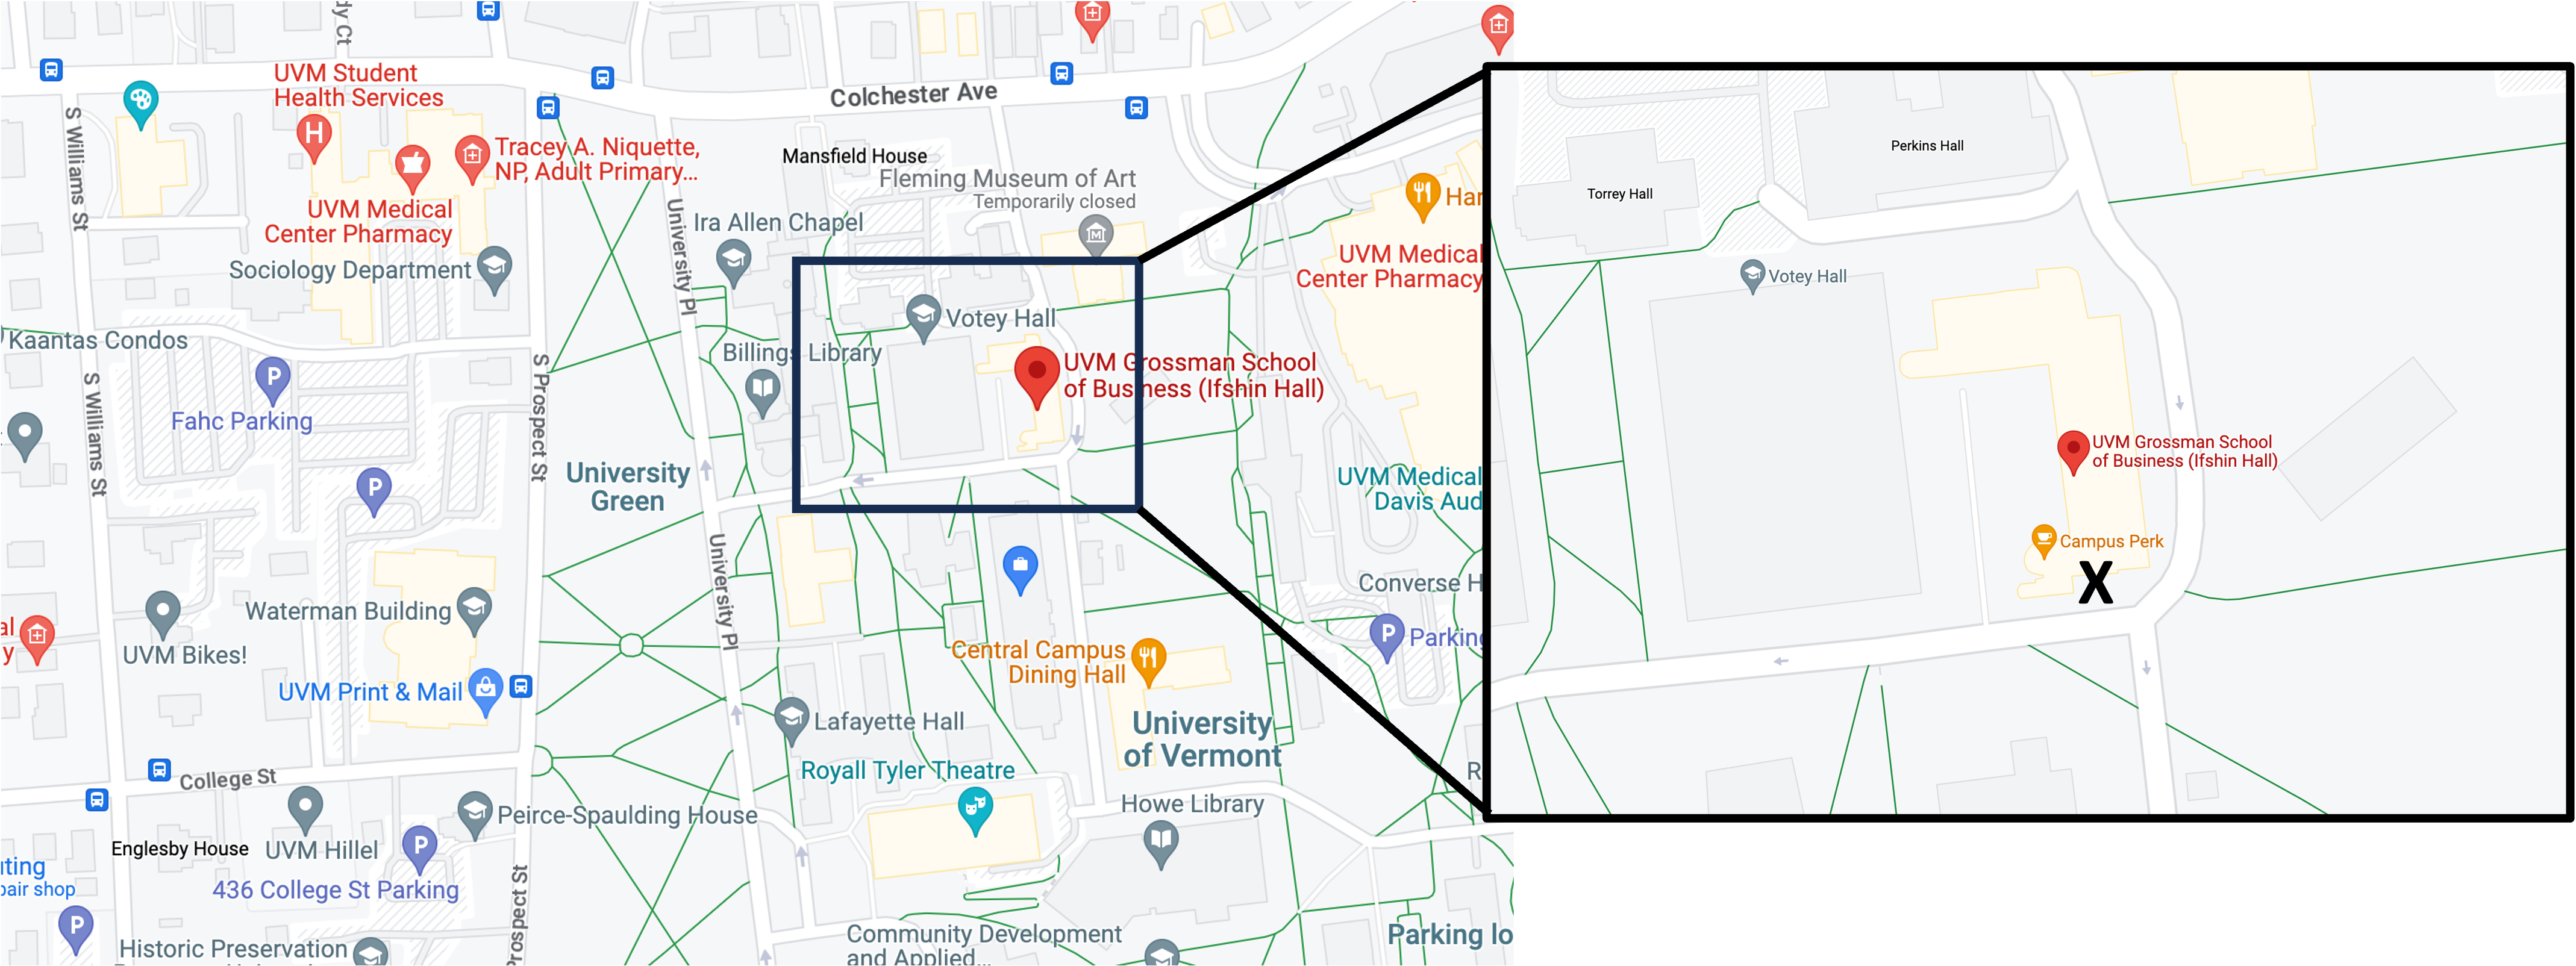
\includegraphics[width=\textwidth]{images/map.png}


\section{Food Recommendations}

\subsection{Breakfast}

\begin{itemize}
    \item Willow's Bagels: allergy friendly options, order ahead to beat the line
    \item The Café Hot: Vegetarian breakfast sandwiches, donuts
    \item The Skinny Pancake: The creperie chain of Vermont
    \item Black Cap: Nice sandwiches, scones, and coffee.
\end{itemize}

\subsection{Lunch}

\begin{itemize}
    \item Folino's: allergy friendly options, order ahead to beat the line
    \item Zabby's: Buffet by weight
    \item Pokeworks: Poke bowls
    \item Pingala Cafe: Vegan food and not too far
    \item Masala Elaichi: Indian food and pretty close to campus
    \item Four Corners of the Earth: Legendary if you can wait a while
    \item Davis Center: Closest option with standard soup/sandwich options
    \item Kampus Kitchen: Sandwiches in a convenience store pretty close to campus
\end{itemize}

\subsection{Dinner}

\begin{itemize}
    \item Folino's (Yep, it's good.)
    \item Citizen Cider: Lots of allergy friendly options
    \item Sherpa Kitchen: Nepalese food
    \item Istanbul Kebab House
\end{itemize}

\subsection{After Dinner}

\begin{itemize}
    \item Burlington Bay: Creemees
    \item Little Gordo Creemee Stand: Self-explanatory
    \item Wallflower Collective: Bar
    \item JP's: The place to go for foosball and Karaoke
\end{itemize}


% % SPONSORS
% %------------------------------------------------------------------
\chapter{Sponsors and Partners}

\section{Sponsors}

\begin{center}
The CCSS 2023 workshop is sponsored by NSF grant \href{https://www.nsf.gov/awardsearch/showAward?AWD_ID=2309867}{2309867}.
\end{center}

\vfill

\section{Partners}

\begin{center}

\includegraphics[width=0.5\textwidth]{images/logos/vcsc.png}

\includegraphics[width=0.5\textwidth]{images/logos/tgir.png}
\end{center}

\vfill

\newpage

% % BACK PAGE
%-----------------------------------------------------------------

\pagecolor{myblue}
\thispagestyle{empty}
\mbox{}

\end{document}